%Ultimatives Tool zur Datierung:
%https://www.cc.kyoto-su.ac.jp/~yanom/pancanga/
%skp = ignored in edition
%skm = ignored in xml
\documentclass[10pt]{memoir}
\setstocksize{220mm}{155mm} 	        
\settrimmedsize{220mm}{155mm}{*}	
\settypeblocksize{170mm}{116mm}{*}	
\setlrmargins{18mm}{*}{*}
\setulmargins{*}{*}{1.2}
%\setlength{\headheight}{5pt}%
\checkandfixthelayout[lines]
\linespread{1.16}
\flushbottom

%%% Hyphenation settings
\usepackage[htt]{hyphenat}
\hyphenation{he-lio-trope opos-sum}
\tracingparagraphs=1
%Hyphenation in Devanāgarī of the edition still missing? Probably this needs to be modified in babel-iast package? 

%%% babel
\usepackage[english]{babel}
\usepackage{babel-iast/babel-iast}

\babelfont[iast]{rm}[Renderer=Harfbuzz, Scale=1.3]{AdishilaSan}%AdishilaSan}
\babelfont[english]{rm}{Adobe Text Pro}

%%% more functionality
\PassOptionsToPackage{hyphens}{url}
\usepackage{hyperref}
\usepackage{pdflscape}
\usepackage{cleveref}
\usepackage{url}
\usepackage{cleveref}
\usepackage{microtype}
\usepackage{lineno}

%\usepackage{bigfoot}
%%% more functions
\usepackage[dvipsnames]{xcolor}
%\usepackage[para,perpage]{footmisc}

%%%für den Counter von Kapiteln und Sätzen! 
\newcommand{\uproman}[1]{\uppercase\expandafter{\romannumeral#1}}
\newcommand{\lowroman}[1]{\romannumeral#1\relax}

\makeindex
\newfontfamily\sanskritfont[Script=Devanagari,Mapping=RomDev,Scale=1.1]{Sanskrit2003}
\usepackage{pifont,fourier-orns,lettrine,psvectorian,paralist,enumitem,pdfpages,wrapfig,tabulary,lettrine,longtable}
\setlist[enumerate]{itemsep=0mm}
\usepackage[autostyle]{csquotes}
\usepackage[defaultlines=2,all]{nowidow}
\usepackage{ellipsis,adforn,booktabs,longtable,url,tikz}
\lineskiplimit=-3pt          

\makechapterstyle{IeT}{%
  \chapterstyle{default}
  \renewcommand*{\printchapternonum}{\centering}
  \renewcommand*{\clearforchapter}{\cleartorecto} 
  \aliaspagestyle{chapter}{empty}}
\chapterstyle{IeT}
\setsecnumdepth{none}  \openright  \nouppercaseheads
\settocdepth{subsubsection}

%%%% test better pagebreaks
%\def\fussy{%
%  \emergencystretch\z@
%  \tolerance 200%
%  \hfuzz .1\p@
%  \vfuzz\hfuzz}

%\interfootnotelinepenalty=10000\relax

%\usepackage[maxfloats=256]{morefloats}

%\maxdeadcycles=500

%raggedbottomsectiontrue
%%\checkandfixthelayout


%%%%%%%  biblatex
%\newcommand{\noun}[1]{\textsc{#1}}    %  philosophy-verbose
\usepackage[backend=biber, sorting=nyt, style=verbose]{biblatex} %%%%ORIGINAL TiE
\renewcommand*{\mkbibnamefamily}[1]{\textsc{#1}}


\DeclareFieldFormat{url}{%
  \mkbibacro{URL}\addcolon\space
  \href{#1}{\nolinkurl{\thefield{urlraw}}}}

\DeclareFieldFormat{citeurl}{%
  \href{#1}{\nolinkurl{\thefield{urlraw}}}} 


\DeclareFieldFormat{postnote}{#1}
\renewcommand{\postnotedelim}{, }
\addbibresource{bindu.bib}

%%% ekdosis
\usepackage[teiexport=tidy,parnotes=true]{ekdosis}% =tidy cleans up HTML and XML documents by fixing markup errors and upgrading legacy code to modern standards. parnotes=footnotes below or above critical apparatus

\SetLineation{lineation=page, modulo} %lineation=page sets thenumbering to start afresh at the top of each page. =modulo makes every fifth line numbered. {lineation=page} makes every line numbered! 

\renewcommand{\linenumberfont}{\selectlanguage{english}\footnotesize} %sets language of lines to English

\SetTEIxmlExport{autopar=false} %autopar=falseinstructs ekdosis to ignore blank lines in the.tex sourcefile as markers for paragraph boundaries. As a result, each paragraph of the edition must be found within an environment associated with the xml <p> element

\SetHooks{
  lemmastyle=\bfseries,
  %refnumstyle=\selectlanguage{english}\bfseries,
  refnumstyle=\selectlanguage{english}\color{blue}\bfseries,
  appheight=0.8\textheight,
}

\newif\ifinapparatus
\DeclareApparatus{source}[
%bhook=\inapparatustrue,
lang=english,
notelang=english,
% bhook=\selectlanguage{english},
bhook=\selectlanguage{english}\textbf{Sources:},%
%maxentries=4, 
%ehook=.]
%sep={] },
%nosep,
]

\newif\ifinapparatus
\DeclareApparatus{testium}[
%bhook=\inapparatustrue,
lang=english,
notelang=english,
% bhook=\selectlanguage{english},
bhook=\selectlanguage{english}\textbf{Testimonia:},
%maxentries=4, 
%ehook=.]
%nosep, 
]

% Declare \ifinapparatus and set \inapparatustrue at the beginning of
% the apparatus criticus block. Also set the language.  
\newif\ifinapparatus
  \DeclareApparatus{default}[
  %bhook=\inapparatustrue, 
  lang=english,
  %maxentries=33,
  %bhook=\selectlanguage{english},
  sep = {] },
  delim=\hskip 0.75em,
  rule=\rule{0.7in}{0.4pt},
]

\newif\ifinapparatus
\DeclareApparatus{philcomm}[
%bhook=\inapparatustrue,
lang=english,
notelang=english,
bhook=\selectlanguage{english}\textbf{Philological Commentary:},
%bhook=\selectlanguage{english},
sep={: },
]

\ekdsetup{
showpagebreaks,
spbmk = \textcolor{blue}{spb},
hpbmk = \textcolor{red}{hpb}
}

%\usepackage{fnpos}
%\makeFNmid
%\makeFNbottom
\usepackage[bottom]{footmisc}
%%%%%%%%%%%%%%%%%%%%%%%%%%%
\makeatletter
\def\blfootnote{\gdef\@thefnmark{}\@footnotetext}
\makeatother
%%%%%%%%%%%%%%%%%%%%%%%%%


% Macros and Definitions for the Print of Sigla
\def\acpc#1#2#3{{#1}\rlap{\textrm{\textsuperscript{#3}}}\textsubscript{\textrm{#2}}\space}
\def\sigl#1#2{{{#1}}\textsubscript{\textrm{#2}}}
\def\None{{\sigl{N}{1}}} \def\Noneac{\acpc{N}{1}{ac}\,} \def\Nonepc{\acpc{N}{1}{pc}\,}
\def\Ntwo{{\sigl{N}{2}}} \def\Noneac{\acpc{N}{2}{ac}\,} \def\Nonepc{\acpc{N}{2}{pc}\,}
\def\Done{{\sigl{D}{1}}} \def\Doneac{\acpc{D}{1}{ac}\,} \def\Donepc{\acpc{D}{1}{pc}\,}
\def\Dtwo{{\sigl{D}{2}}} \def\Dtwoac{\acpc{D}{2}{ac}\,} \def\Dtwopc{\acpc{D}{2}{pc}\,}
\def\Uone{{\sigl{U}{1}}} \def\Uoneac{\acpc{U}{1}{ac}\,} \def\Uonepc{\acpc{U}{1}{pc}\,}                 
\def\Utwo{{\sigl{U}{2}}} \def\Utwoac{\acpc{U}{2}{ac}\,} \def\Utwopc{\acpc{U}{2}{pc}\,}

%%%%%%%%%%%%%% Tattvabinduyoga - List of Witnesses   %%%%%%%%%%%%%%%%%%%
\DeclareWitness{ceteri}{\selectlanguage{english}cett.}{ceteri}[]   
\DeclareWitness{E}{\selectlanguage{english}E}{Printed Edition}[]    
\DeclareWitness{P}{\selectlanguage{english}P}{Pune BORI 664}[]  
\DeclareWitness{B}{\selectlanguage{english}B}{Bodleian 485}[]       
\DeclareWitness{N1}{\selectlanguage{english}N\textsubscript{1}}{NGMPP 38/31}[]
\DeclareWitness{N2}{\selectlanguage{english}N\textsubscript{2}}{NGMPP B 38/35}[]
\DeclareWitness{L}{\selectlanguage{english}L}{LALCHAND 5876}[]  
\DeclareWitness{D}{\selectlanguage{english}D}{IGNCA 30019}[] 
%\DeclareWitness{D2}{\selectlanguage{english}D\textsubscript{2}}{IGNCA 30020}[]  
\DeclareWitness{U1}{\selectlanguage{english}U\textsubscript{1}}{SORI 1574}[] 
\DeclareWitness{U2}{\selectlanguage{english}U\textsubscript{2}}{SORI 6082}[]
%%%%%%%%%%%%%% Tattvabinduyoga - Groups of Witnesses   %%%%%%%%%%%%%%%%%%%
\DeclareWitness{X}{\selectlanguage{english}\alpha}{Alpha Group: D,N1,N2,U1}[]
\DeclareWitness{Y}{\selectlanguage{english}\beta}{Beta Group: B,E,L,P,U2}[]
%%%%%%%%%%%%% Testimonia
\DeclareWitness{Ysv}{\selectlanguage{english}Ysv}{Yogasvarodaya}[] %%%add infos!  

%%%%%%%%%%%%%%%%%%%%%%%%%%%%%%%%%%%%%%%%%%%
% Macro for Editing Abbrevs.
\def\om{\textrm{\footnotesize \textit{om.}\ }} %prints om. for omitted in apparatus
\def\korr{\textrm{\footnotesize \textit{em.}\ }} %prints em. for emended in apparatus
\def\conj{\textrm{\footnotesize \textit{conj.}\ }} %prints conj. for conjectured in apparatus

% \supplied{text} EDITORIAL ADDITION -> Within \lem oder \rdg
% \surplus{text} EDITORIAL DELETION -> Within \lem oder \rdg
% \sic{text} CRUX
% \gap{text} LACUNAE -> [reason=??, unit=??, quantity=??, extent=??]


%%%%%%%%%%%%%%%%%%%%%%%%%%%%%%%%%%%%%%%%%%% All macros of this list can be used in 
% Macro for Editing Abbrevs.
\def\eyeskip{\textrm{{ab.\,oc. }}}
\def\aberratio{\textrm{{ab.\,oc. }}}
\def\ad{\textrm{{ad}}}
\def\add{\textrm{{add.\ }}}
\def\ann{\textrm{{ann.\ }}}
\def\ante{\textrm{{ante }}} 
\def\post{\textrm{{post }}}
%\def\ceteri{cett.\,}                   
\def\codd{\textrm{{codd.\ }}}

\def\coni{\textrm{{coni.\ }}}
\def\contin{\textrm{{contin.\ }}}
\def\corr{\textrm{{corr.\ }}}
\def\del{\textrm{{del.\ }}}
\def\dub{\textrm{{ dub.\ }}}

\def\expl{\textrm{{explic.\ }}} 
\def\explica t{\textrm{{explic.\ }}}
\def\fol{\textrm{{fol.\ }}}
\def\foll{\textrm{{foll.\ }}}
\def\gloss{\textrm{{glossa ad }}}
\def\ins{\textrm{{ins.\ }}}      
\def\inseruit{\textrm{{ins.\ }}} 
\def\im{{\kern-.7pt\lower-1ex\hbox{\textrm{\tiny{\emph{i.m.}}}\kern0pt}}} %\textrm{\scriptsize{i.m.\ }}}      
\def\inmargine{{\kern-.7pt\lower-.7ex\hbox{\textrm{\tiny{\emph{i.m.}}}\kern0pt}}}%\textrm{\scriptsize{i.m.\ }}}      
\def\intextu{{\kern-.7pt\lower-.95ex\hbox{\textrm{\tiny{\emph{i.t.}}}\kern0pt}}}%\textrm{\scriptsize{i.t.\ }}}           
\def\indist{\textrm{{indis.\ }}}  
\def\indis{\textrm{{indis.\ }}}
\def\iteravit{\textrm{{iter.\ }}} 
\def\iter{\textrm{{iter.\ }}}
\def\lectio{\textrm{{lect.\ }}}   
\def\lec{\textrm{{lect.\ }}}
\def\leginequit{\textrm{{l.n. }}} 
\def\legn{\textrm{{l.n. }}}
\def\illeg{\textrm{{l.n. }}}

\def\primman{\textrm{{pr.m.}}}
\def\prob{\textrm{{prob.}}}
\def\rep{\textrm{{repetitio }}}
\def\secundamanu{\textrm{\scriptsize{s.m.}}}            \def\secm{{\kern-.6pt\lower-.91ex\hbox{\textrm{\tiny{\emph{s.m.}}}\kern0pt}}}%   \textrm{\scriptsize{s.m.}}}
\def\sequentia{\textrm{{seq.\,inv.\ }}}  
\def\seqinv{\textrm{{seq.\,inv.\ }}}
\def\order{\textrm{{seq.\,inv.\ }}}
\def\supralineam{{\kern-.7pt\lower-.91ex\hbox{\textrm{\tiny{\emph{s.l.}}}\kern0pt}}} %\textrm{\scriptsize{s.l.}}}
\def\interlineam{{\kern-.7pt\lower-.91ex\hbox{\textrm{\tiny{\emph{s.l.}}}\kern0pt}}}   %\textrm{\scriptsize{s.l.}}}
\def\vl{\textrm{v.l.}}   \def\varlec{\textrm{v.l.}} \def\varialectio{\textrm{v.l.}}
\def\vide{\textrm{{cf.\ }}}
\def\cf{\textrm{{cf.\ }}} 
\def\videtur{\textrm{{vid.\,ut}}}
\def\crux{\textup{[\ldots]} }
\def\cruxx{\textup{[\ldots]}}
\def\unm{\textit{unm.}}
%%%%%%%%%%%%%%%%%%%%%%%%%%%%%%%%%%%%

% List of Scholars
\DeclareScholar{ego}{ego}[
forename=Nils Jacob,
surname=Liersch]

% Persons:14\DeclareScholar{ego}{ego}[15forename=Robert,16surname=Alessi]17% Useful shorthands:18\DeclareShorthand{codd}{codd.}{V,I,R,H}19\DeclareShorthand{edd}{edd.}{Lit,Erm,Sm}20\DeclareShorthand{egoscr}{\emph{scripsi}}{ego}

%Useful shorthands:
%\DeclareShorthand{codd}{codd.}{V,I,R,H}
%\DeclareShorthand{edd}{edd.}{Lit,Erm,Sm}
\DeclareShorthand{egoscr}{em.}{ego}
\DeclareShorthand{egoscrconj}{conj.}{ego}
\DeclareShorthand{egomute}{\unskip}{ego}

\usepackage{xparse}

\NewDocumentEnvironment{tlg}{O{}O{}}{\setlength{\leftskip}{0pt}\vspace{-1ex}\begin{quotation}}{\hfill #1\ \vspace{-1ex}\end{quotation}\vspace{-1ex}} %verse environment
%\NewDocumentEnvironment{tlg}{O{}O{}}{\begin{verse}}{॥#1\hskip-4pt ॥\\ \end{verse}}
\NewDocumentCommand{\tl}{m}{{\selectlanguage{iast} #1}}

\NewDocumentCommand{\extra}{m}{{\textcolor{gray}{#1}}} %command for additions to U2
\NewDocumentCommand{\crazy}{m}{{\textcolor{red}{#1}}} %totally corrupted passage
\NewDocumentCommand{\coro}{m}{{\textcolor{violet}{#1}}} %colour for sentence counter! 

\NewDocumentEnvironment{prose}{O{}}{\begin{otherlanguage}{iast}}{\end{otherlanguage}}
% \NewDocumentEnvironment{padd}{O{}}{\begin{otherlanguage}{iast}}{\end{otherlanguage}}
\NewDocumentEnvironment{tlate}{O{}}
%\NewDocumentEnvironment{tadd}{O{}}

%Define two commands: \skp ("sanskrit plus"), to be ignored by TeX in
%the edition text, but processed in the TEI output. Conversely, \skm
%("sanskrit minus") is to be processed in the edition text, but
%ignored if found in the apparatus criticus and in the TEI output:

\NewDocumentCommand{\skp}{m}{}
\TeXtoTEIPat{\skp {#1}}{#1}

%\NewDocumentCommand{\skpp}{m}{}
%\TeXtoTEIPat{\skpp {#1}}{#1}

\NewDocumentCommand{\skm}{m}{\unless\ifinapparatus#1-\fi}
\TeXtoTEIPat{\skm {#1}}{}

% \NewDocumentCommand{\dd}{}{/\hskip-4pt/}
\NewDocumentCommand{\dd}{}{\mbox{/\hskip-4pt/}}
\TeXtoTEIPat{\dd {}}{//}


%%% modify environments and commands
%%% TEI mapping
\TeXtoTEIPat{\begin {tlg}}{<lg>} %lg=(Group of verse (s)) contains one or more verses or lines of verse that together form a formal unit (e.g. stanza, chorus).
\TeXtoTEIPat{\end {tlg}}{</lg>}

\TeXtoTEIPat{\begin {prose}}{<p>}
\TeXtoTEIPat{\end {prose}}{</p>}

\TeXtoTEIPat{\begin {tlate}}{<p>}
\TeXtoTEIPat{\end {tlate}}{</p>}

\TeXtoTEIPat{\\}{}
\TeXtoTEIPat{\linebreak}{<br/>}
\TeXtoTEIPat{\noindent}{}
%\TeXtoTEI{tl}{l}
\TeXtoTEI{emph}{hi}
\TeXtoTEI{bigskip}{}
\TeXtoTEI{None}{N1}
\TeXtoTEI{Ntwo}{N2}
\TeXtoTEI{Done}{D1}
\TeXtoTEI{Dtwo}{D2}
\TeXtoTEI{Uone}{U1}
\TeXtoTEI{Utwo}{U2}
%\TeXtoTEIPat{/}{ |}
%\TeXtoTEI{//}{ ||}
\TeXtoTEIPat{\korr}{em. }
\TeXtoTEIPat{\conj}{conj.}
\TeXtoTEIPat{\om}{om.}
\TeXtoTEIPat{english}{}
\TeXtoTEIPat{\hskip}{}
\TeXtoTEIPat{\hskip-4pt}{}
\TeXtoTEIPat{\hskip-2pt}{}
\TeXtoTEIPat{-}{ }
\TeXtoTEIPat{4pt}{}
\TeXtoTEIPat{2pt}{}
\TeXtoTEIPat{\textcolor {#1}{#2}}{<hi rend="#1">#2</hi>} 

% Nullify \selectlanguage in TEI as it has been used in
% \DeclareWitness but should be ignored in TEI.
\TeXtoTEI{selectlanguage}{}



\FormatDiv{1}{\begin{center}\Large}{\end{center}}
\FormatDiv{2}{\begin{center}\small}{\end{center}}
\FormatDiv{3}{\bfseries}{.}
\title{Tattvayogabindu of Rāmacandra\\ A Critical Edition and Annotated Translation\\ and a Comparative Analysis of the \\Complex Early Modern Yoga Yaxonomies }
\date{\today}
\parindent=15pt

\begin{document}

\frontmatter
\thispagestyle{empty} % Verhindert Seitenzahl auf der Seite
\begin{center}

%\vspace{0.5in}

%\begin{otherlanguage}{iast}
%   \large\sanskritfont{Tattvayogabindu}\\
%\end{otherlanguage}

\vspace{0.25in}


\huge\textbf{\MakeUppercase{The Tattvayogabindu \\of Rāmacandra}}\\

\vspace{0.2in}

\Large  Critical Edition and Annotated Translation of an Early Modern Text on Rājayoga, with a Comparative Analysis of the Complex Yoga Taxonomies from the Same Period\\ 

\vspace{0.45in}

\thispagestyle{empty}
\end{center}
%\newpage
%\thispagestyle{empty}
%\mbox{}
%\newpage

\newpage

  \thispagestyle{empty}
  \begin{figure}[p]
    \centering
    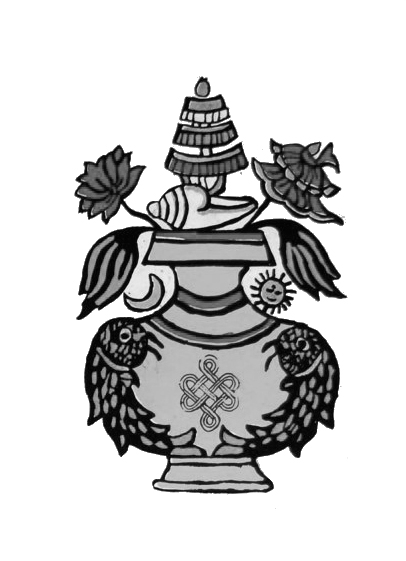
\includegraphics[width=0.25\textwidth]{pics/purna.jpg}
  \end{figure}
  
\newpage

\begin{landscape}
\thispagestyle{empty}
  \begin{figure}[p]
	\centering
  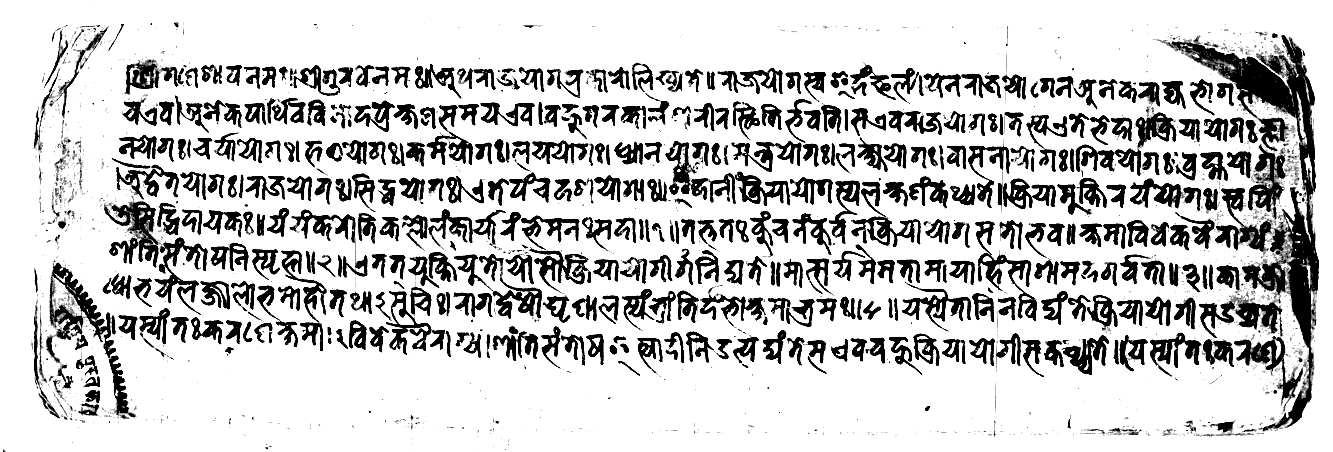
\includegraphics[width=1.5\textwidth]{pics/folio1.jpg}
	\caption{Folio 1v of Ms. \getsiglum{N1}.}
	 \phantomsection\label{fig_folio1}
\end{figure}
\end{landscape}

\cleardoublepage
\tableofcontents
\thispagestyle{empty}
\newpage 
\listoffigures
\thispagestyle{empty}
\newpage
\listoftables
\thispagestyle{empty}
\newpage

\mainmatter
\pagestyle{defaultstyle}
\counterwithout{footnote}{chapter}
\counterwithout{figure}{chapter}
\counterwithout{table}{chapter}
\renewcommand{\thetable}{\arabic{table}}
%%%tables 
\setsecnumdepth{section}
\maxsecnumdepth{subsubsection}
\newpage
\chapter{Introduction}
\cleardoublepage

\section{General remarks}
 \phantomsection\label{generalremarks}
 \lettrine{T}{he} \textit{Tattvayogabindu} of Rāmacandra\footnote{A discussion about the author Rāmacandra is found on p. \pageref{ramarama}.} is an early modern Sanskrit text on Rājayoga that was written in the first half of the seventeenth century\footnote{The dating of the text is discussed on p. \pageref{dating}.} in northern India.\footnote{The detailed discussion of the place of origin is found on p. \pageref{riversrivers}, n. \ref{riversrivers}.} The most salient feature of the work that makes it historically significant is its highly differentiated taxonomy of types of yoga.\footnote{This is a remarkable increase in the number of declared yogas compared to the standard medieval tetrad of Mantra, Laya, Haṭha and Rājayoga.} In the \textit{Tattvayogabindu}'s introduction, most manuscripts name fifteen types of yoga, presented as methods of Rājayoga. These are 1. Kriyāyoga, 2. Jñānayoga, 3. Caryāyoga, 4. Haṭhayoga, 5. Karmayoga, 6. Layayoga, 7. Dhyānayoga, 8. Mantrayoga, 9. Lakṣyayoga, 10. Vāsanāyoga, 11. Śivayoga, 12. Brahmayoga, 13. Advaitayoga, 14. Siddhayoga, and 15. Rājayoga itself. The text is a yogic compendium written in a mix of mainly prose and 47 verses in textbook-style, where its 59 topics are introduced in sections most of the time launched by recognizable phrases. The sections deal with the methods of Rājayoga and their effects, but others also cover topics like yogic physiology, the Avadhūta, the importance of the guru, cosmogony, and a \textit{yogaśāstrarahasya}.  

The \textit{Tattvayogabindu} has not been discussed comprehensively or considered in the secondary literature on yoga. The only exception is \citeauthor{birch2014} (2014: 415–416) who briefly described its list of fifteen yogas in the context of the ``fifteen medieval yogas'' and noted that a similar taxonomy occurs in Nārāyaṇatīrtha’s \textit{Yogasiddhāntacandrikā} (17th century), a commentary on the \textit{Pātañjalayogaśāstra} that integrates fifteen medieval yogas within its \textit{aṣṭāṅga} format. An incomplete account of the fifteen yogas is found within the Sanskrit yoga text \textit{Yogasvarodaya}, which is known only through quotations in the \textit{Prāṇatoṣinī}, the \textit{Yogakarṇikā} and the \emph{Śabdakalpadruma}.\footnote{Manuscripts under the name of \textit{Yogasvarodaya} seem to be lost. I was not able to locate the manuscripts of the text in any manuscript catalogue at hand.} The \textit{Yogasvarodaya} announces a total of fifteen yogas but names only eight of them in its introductory \textit{śloka}s. It is the primary source and template for the compilation of the \textit{Tattvayogabindu}. Besides several passages, Rāmacandra, in many instances, follows its content and structure by rewriting the \textit{Yogasvarodaya}’s \textit{śloka}s into prose or quoting them directly without attribution. Due to the incomplete transmission of the \textit{Yogasvarodaya}, Rāmacandra’s \textit{Tattvayogabindu} is a natural and valuable starting point for an unprecedented in-depth study of the complex early modern yoga taxonomies, a phenomenon that can be narrowed down precisely in terms of time and as I will show regarding its localisation. The other source text that Rāmacandra used is the \textit{Siddhasiddhāntapaddhati} whose content he draws on, particularly in the second half of his composition. Another text that includes an almost similar taxonomy of twelve yogas divided into three tetrads\footnote{See p.\pageref{sarvasarva} for a detailed discussion of the \textit{Sarvāṅgayogapradīpikā}.} is Sundardās’s \textit{Brajbhāṣā} yoga text named \textit{Sarvāṅgayogapradīpikā} which not just shares most of the types of yogas but also provides a different and valuable perspective on the addressed yoga categories.\footnote{For a comparative table of the complex early modern yoga taxonomies see table \ref{tab:complextaxonomies} on p. \pageref{tab:complextaxonomies}.}

These complex taxonomies that emerged during the 17th century crossed sectarian divides and were adapted to the specific needs of different authors and traditions. The \textit{Tattvayogabindu} thus encapsulates a large proportion of the diversity of yoga types and teachings after the \textit{Haṭhapradīpikā} (15th century) that were adopted and practised by a broad spectrum of religious traditions and strata of Indian society. In the particular case of the \textit{Tattvayogabindu}, there are various statements throughout the text that reveal a strategy to detach yoga from its ascetic and renunciate connotations and to stylise Rājayoga as a practice that can bring the desired soteriological benefits even to practitioners who enjoy worldly pleasures and expensive lifestyles. Textual evidence suggests that the \textit{Tattvayogabindu} is an important example of a text that provides an early modern adaptation of Rājayoga for \textit{kṣatriya}s in a courtly environment.

One printed edition of the \textit{Tattvayogabindu} was published in 1905 with a Hindi translation and based on (an) unknown manuscript(s).\footnote{\emph{Binduyoga}. \textit{Binduyogaḥ with Bhāṣaṭīkā}. Ed. by Jvālāprasāda Miśra. Mumbai, 1905.} This publication has the title ``\textit{Binduyoga}'' confirmed by the printed text’s colophon. However, as I will discuss in the introduction, the text was originally known as \textit{Tattvayogabindu}. The consulted manuscripts contain significant discrepancies, structural differences and variant readings between them and the printed edition.\footnote{For example, the printed edition does not contain the complex yoga taxonomy presented in the manuscripts of the \emph{Tattvayogabindu}.} Furthermore, the manuscripts are scattered over the northern half of the Indian subcontinent and Nepal, which suggests that the text was widely transmitted at some point. Lengthy passages of the \textit{Tattvayogabindu} are quoted without attribution in a text called \textit{Yogasaṃgraha} and Sundaradeva’s \textit{Haṭhasaṅketacandrikā}.

The first chapter of this dissertation contains a general introduction to Rāmacandra's \textit{Tattvayogabindu}. The chapter gives a brief overview of the content of the text and discusses its origin, the author and the author's intended audience. Subsequently, the textual witnesses, source texts and testimonies of the \textit{Tattvayogabindu} are described. A stemmatic analysis of the text is then presented, based on manual philological observation and computer-assisted stemmatics to present a \textit{stemma codicum}. The chapter concludes with a presentation of the editorial policies, which form the basis for the second chapter of this thesis.
The second chapter, the core of this dissertation, is a critical edition and annotated translation of the \textit{Tattvayogabindu}. The critical edition significantly improves the text and sheds new light on its historical significance.
The third chapter contains a comparative analysis of the complex early modern yoga taxonomies based on hermeneutics of difference.\footnote{The conceptof hermeneutics of difference is discussed on p. \pageref{hermeneutics}, n. \ref{hemerneutics}.}  Using the new critical edition of the \textit{Tattvayogabindu} and the texts mentioned above, \emph{Yogasvarodaya}, \emph{Yogasiddhāntacandrikā} and \emph{Sarvāṅgayogapradīpikā}, the complex yogic taxonomies of the four texts are compared in detail. Based on this comparative analysis, a differentiated hypothesis on the emergence of the complex yoga taxonomies was developed, and the complex yoga taxonomies were located und explained in the broader context of the historical development of the yoga traditions. The comparison includes a nuanced description of each yoga category used by the authors of the texts with complex yoga taxonomies. While the authors of the four texts often operate with identical terms for the individual yoga categories, they interpret these categories according to their religious backgrounds and agendas, with intriguing and exciting differences. Contrasting the comparanda, i.e. the authors, the texts, the yoga taxonomies and the yoga categories, therefore provides a deep insight into the discursive negotiation processes of the Indian yoga traditions of the 17th century.


\chapter{Conventions in the Critical Apparatus}
\section{Sigla in the Critical Apparatus}

\begin{itemize}
\item \beta : \getsiglum{D}, \getsiglum{J}, \getsiglum{K1}, \getsiglum{N1}, \getsiglum{N2}, \getsiglum{U1}
\item \gamma : \getsiglum{B}, \getsiglum{E}, \getsiglum{L}, \getsiglum{P}, \getsiglum{U2}
\item B : Bodleian Oxford D 4587
\item C : \emph{Haṭhasaṅketacandrikā} GOML Ms. No. R 3239
\item C\textsubscript{pc} : \emph{Haṭhasaṅketacandrikā} GOML Ms. No. R 3239
\item cett.: ceteri (all manuscripts except the ones mentioned in the lemma)
\item \Done : IGNCA 30019
\item E : Printed Edition
\item J : JNUL Ms. No. 55769
\item Jo : \emph{Haṭhasaṅketacandrikā} MMPP MS. No. 2244
\item \Kone : AS G 11019
\item L : Lalchand Research Library LRL5876
\item M : \emph{Haṭhasaṅketacandrikā} ORI Ms. No. B 220
\item \Ntwo : NGMPP B 38-35 / A 1327-14
\item \None : NGMPP B 38-31
\item P : Pune BORI 664
\item PT : \emph{Prāṇatoṣiṇī}
\item \Uone : SORI 1574
\item \Utwo : SORI 6082
\item V : OI MSU 10558
\item YK : \emph{Yogakarṇikā}% 
\item YSv : \emph{Yogasvarodaya}
\end{itemize}
\newpage

\chapter[Critical Edition \& Annotated Translation of the \emph{Tattvayogabindu}]{The \emph{Tattvayogabindu} of Rāmacandra \\ \huge  
  Critical Edition \& Annotated Translation}
\pagestyle{chapter2style}
\cleardoublepage
\begin{alignment}[
    texts=edition[class="edition"];
    translation[class="translation"],
  ]
  \begin{edition}
    \begin{prose}[p03_2]
      \noindent
 \note[type=source, labelb=_9b, labele=_9e, nosep]{cf. YSv (PT, p. 831): paṭhanāt smaraṇād vyānān maṇḍanāt brahmasādhakaḥ | tad bhedasyaikasandhānam aṣṭaiśvaryamayo bhavet | tritīrthaṃ yatra nāḍī ca tripuṇyaṃ parameśvari | \ldots eṣo 'sya viśvarūpasya rājayogo mato budhaiḥ | viśeṣaṃ kathayiṣyāmi śṛṇu caikamanāḥ sati | mūlakande sthale caikā nāḍī tejasvatī parā (\textit{tejasvitāparā} YK 1.246) |  gudorddhe (\textit{gudordhve} YK 1.247) sā tribhāgābhūd iḍā (\textit{tridhā bhūyād iḍā vāme} YK 1.247) nāma śaśiprabhā | śaktirūpā mahānāḍī dhyānāt sarvārthadāyinī | dakṣiṇe 'pi kulākhyeti (\textit{dakṣiṇe piṅgalākhyeti} YK 1.248) puṃrūpā sūryavigrahā |  madhyabhāge suṣumnākhyā brahmaviṣṇuśivātmikā | śuddhacittena sā vijñā vidyutkoṭisamaprabhā | bhuktimuktipradā dhyānād aṇimādiguṇapradā | suṣumnāntaḥ samāśritya navacakraṃ yathā śṛṇu | mūlādhāraṃ catuṣpatraṃ gudorddhe (\textit{gudordhve} YK 1.250) varttate mahat}
 \note[type=testium, labelb=_9b, labele=_9e, nosep]{ \approx  \textit{Yogasaṃgraha} (IGNCA 30020 f. 2v. ll. 3-7): mūlakandasthāne ekā tejomayā mahānāḍī vartate | iyaṃ iḍāpiṅgalasuṣumnā bhedā tridhā | vāma\-bhāge candrarūpā iḍā | dakṣiṇabhāge sūryarūpā piṅgalā |  madhyamārge atisūkṣmā visataṃtusamākārā koṭividyutprabhā bhuktimuktipradā suṣumnā nāḍī vartate | yasyāḥ jñāne puruṣaḥ sarvajño bhavati | atas taj jñānotpattāv upāyā ucyaṃte | gudamūlacakraṃ caturdalaṃ |}
 \note[type=source, labelb=_9b, labele=_9e, nosep]{cf. SSP 2.26 (Ed. p. 38): mūlakandād daṇḍalagnāṃ brahmanāḍīṃ śvetavarṇāṃ brahmarandhraparyantaṃ gatāṃ saṃsmaret | tanmadhye kamalatantunibhāṃ vidyutkoṭiprabhām ūrdhvagāminīṃ tāṃ mūrtiṃ manasā lakṣayet | sarvasiddhipradā bhavati | piṇḍe navacakrāṇi | ādhāre brahmacakraṃ tridhāvartaṃ bhagamaṇḍalākāram | tatra mūlakandaḥ |}
%-----------------------
% \om                         \B
%astu rājayogaḥ kathyate/    \E
%amū  rājayogau kathyete       \P
%amū  rājayogau kathyate//    \L
%amū  rājayogau kathyate       \N1
%amū  rājayogau kathyate//     \N2  %%%p3verso
%amū  rājayogau kathyate//    \D
%amū  rājayogau kathyate//    \J       
%amū  rājayogau kathyate//    \K1
%amū  rājayogau kathyate       \U1
%amū  rājayogau kathyaṃte//   \U2
%-----------------------
%These two rājayogas are described [in the following].
%-----------------------
       \app{\lem[wit={ceteri}]{amū}\linelabel{_9b}
         \rdg[wit={E}]{astu}}
       rāja\app{\lem[wit={ceteri}, alt={°yogau}]{yogau}
         \rdg[wit={E}]{°yogaḥ}}
       \app{\lem[wit={P}]{kathyete}
         \rdg[wit={X,E,L}]{kathyate}
         \rdg[wit={U2}]{kathyaṃte}}/
%-----------------------
% \om                                                              \B
%mūlakandasthāne    ekā tejorūpā    mahānāḍī varttate /            \E
%mūlaṃ kaṃdasthāne  ekā tejorūpā    mahānāḍī varttate              \P
%mūlakaṃdasthāne    ekā tejorūpā    mahānāḍī vartate               \L
%mūlakaṃdasthāne    eka tejorūpā    mahānāḍī varttate /            \N1
%mūlakaṃdasthāne    eka tejorūpā    mahānāḍī varttate /            \N2
%mūlakaṃdasthāne    ekā tejorūpā    mahānāḍī varttate //           \D
%mūlakaṃdasthāne    ekāṃ tejorūpā//    mahānāḍī varttate //           \J       
%mūlakaṃdasthāne    ekā tejorūpā    mahānāḍī varttate //           \K1
%mūlakaṃdasthāne    ekā tejorūpā    mahānāḍī vartate /             \U1
%mūlakaṃdasthāne // ekā tejorūpā // mahānāḍī pravarttate /         \U2
%-----------------------
%At the location of the root-bulb exists one major channel in the form of light.
%-----------------------       
       mūla\app{\lem[wit={ceteri}, alt={°kandasthāne}]{kandasthāne}
         \rdg[wit={U2}]{°kaṃdasthāne ||}
         \rdg[wit={P}]{°ṃ kaṃdasthāne}}
       \app{\lem[wit={ceteri}]{ekā}
         \rdg[wit={J}]{ekāṃ}
         \rdg[wit={N1,N2}]{eka}}
       tejorūpā mahānāḍī
       \app{\lem[wit={ceteri}]{vartate}
         \rdg[wit={U2}]{pravartate}}/
%-----------------------
% \om                                                            \B
%iyam ekanāḍī /  iḍāpiṃgalāsuṣumṇā      etān bhedān prāpnoti /    \E
%iyaṃ ekanāḍī    iḍāpiṃgalāsuṣumṇā      etān bhedān prāpnoti      \P
%trayaṃ kā nāḍī  iḍāpiṃgalāsuṣumnā //   etān bhedān prāpnoti      \L
%iyaṃ ekā nāḍī   iḍāpiṃgalāsuṣumnān /   ete  bhedān prāpnoti      \N1
%iyaṃ ekā nāḍī   iḍāpiṃgalāsuṣumnān//   ete  bhedān prāpnoti/     \N2
%iyaṃ ekā nāḍī   iḍāpiṃgalasuṣumnān //  ete  bhedān prāpnoti      \D
%iyaṃ ekā nāḍī   iḍāpiṃgalasuṣumnā//    etān bhedān prāpnoti/       \J           
%iyaṃ ekā nāḍī   idāpiṃgalasuṣumnān //  ete  bhedān prāpnoti      \K1
%iyaṃ ekā nāḍī   iḍāpiṃgalāsuṣumnā      etān bhedān prāpnoti      \U1
%iyaṃ eka nāḍī   iḍāpiṃgalāsuṣumṇā      etān bhegān prāpnoti      \U2
%-----------------------
% This single channel splits up into \textit{iḍā}, \textit{piṅgalā} and \textit{suṣumnā}.
%-----------------------       
\app{\lem[wit={E},alt={iyam}]{iya\skm{m-e}}
         \rdg[wit={ceteri}]{iyaṃ}
         \rdg[wit={L}]{trayaṃ}
}\app{\lem[wit={ceteri}, alt={ekā}]{\skp{m-e}kā}
         \rdg[wit={E}]{eka |}
         \rdg[wit={P}]{eka}
         \rdg[wit={L}]{kā}}
       nāḍī iḍā\app{\lem[wit={ceteri}, alt={°piṅgalā°}]{piṅgalā}
        \rdg[wit={D,J,K1}]{°piṅgala°}}\app{\lem[type=emendation, resp=egoscr, alt={°suṣumṇān}]{suṣumṇāḥ}
         \rdg[wit={D,K1,N1,N2}]{suṣumnān}
         \rdg[wit={E,P,U2}]{°suṣumṇā}
         \rdg[wit={J,L,U1}]{°suṣumnā}}\dd{}
       \app{\lem[wit={J,Y,U1}]{etān}
         \rdg[wit={D,K1,N1,N2}]{ete}} bhedān prāpnoti/
%-----------------------
%\om                                           \B
%vāmabhāge candrarūpā iḍā nāḍī varttate /      \E
%vāmabhāge caṃdrarūpā iḍā nāḍī varttate        \P
%vāmabhāge caṃdrarūpā iḍā nāḍī varttate //     \L
%vāmabhāge caṃdrarūpā iḍā nāḍī varttate /      \N1
%vāmabhāge caṃdrarūpā iḍā nāḍī varttate //     \N2
%vāmabhāge caṃdrarūpā iḍā nāḍī varttate /      \D
%vāmabhāge caṃdrarūpā iḍā nāḍī varttate //      \J       
%vāmabhāge caṃdrarūpā iḍā nāḍī varttate //      \K1
%vāmabhāge caṃdrarūpā iḍā nāḍī vartate         \U1
%vāmabhāge caṃdrarūpā     nāḍī pravarttate //  \U2
%-----------------------
%On the left side is the lunar \textit{iḍā}-channel.
%-----------------------        
vāmabhāge candrarūpā
        \app{\lem[wit={ceteri}]{iḍā}
          \rdg[wit={U2}]{\om}}nāḍī
        \app{\lem[wit={ceteri}]{vartate}
          \rdg[wit={U2}]{pravarttate}}/
%-----------------------
% \om                                                \B
%dakṣiṇabhāge  sūryarūpā piṅgalā  nāḍī    varttate /  \E
%dakṣiṇabhāge  sūryarūpā piṃgalā  nāḍī    varttate    \P
%dakṣiṇabhāge  sūryarūpā piṃgalā  nāḍī    varttate // \L
%dakṣiṇabhāge  sūryarūpā piṃgalā  nāḍī    varttate // \N1
%dakṣiṇabhāge  sūryarūpā piṃgalā  nāḍī    varttate/   \N2
%dakṣiṇabhāge  sūryarūpā piṃgalā  nāḍī    varttate // \D
%dakṣiṇe bhāge  sūryarūpā piṃgalā  nāḍī    vartate // \J          
%dakṣiṇabhāge  sūryarūpā piṃgalā  nāḍī    varttate // \K1
%dakṣiṇe bhāge sūryarūpā piṃgalā  nāḍī    vartate     \U1
%dakṣiṇabhāge  sūryarūpā piṃgalā  nāḍī pravartate //  \U2
%-----------------------
%On the right side exists the solar \textit{piṅgalā}-channel.        
%-----------------------
        \app{\lem[wit={ceteri}, alt={dakṣiṇa°}]{dakṣiṇa}
          \rdg[wit={J,U1}]{dakṣiṇe}}bhāge
        sūryarūpā piṅgalānāḍī
        \app{\lem[wit={ceteri}]{vartate}
          \rdg[wit={U2}]{pravarttate}}/
%-----------------------
% \om                                                                   \B
%madhyamārge `tisūkṣmā padminītaṃtusamākārā  koṭividyutsamaprabhā      \E
%madhyamārge `tisūkṣmā padmanītaṃtusamākāra  koṭividyutsamaprabhā      \P
%madhyamārge `tisūkṣmā padmanītaṃtusamākārā  koṭividyutsamaprabhā      \L
%madhyamārge atisūkṣmā padmanītaṃtusamākārā  koṭividyutsamaprabhā //   \N1
%madhyamārge atisūkṣmā padmanītaṃtusamākārā  koṭividyutsamaprabhā //   \N2
%madhyarge   atisūkṣmā padminītaṃtusamākārā  koṭividyutsamaprabhā //   \D
%madhyamarge   sūkṣmā  padminītantusamākārā  koṭividyutsamaprabhā   \J        
%madhyamārge atisūkṣmā pa++nyanītaṃtusamākārā  koṭividyutsamaprabhā //   \K1
%madhyamārge atisūkṣmā padminītaṃtusamākārā  koṭividyutsamaprabaḥ      \U1
%madhyamārge  tisūkṣmā padminītaṃtusamākārā  koṭividyutsamaprabhā //   \U2
%-----------------------
%Within the middle path, having the very subtle form equal to the fibre of a stalk of a lotus [and] shining like a thousand lightnings, 
%----------------------- 
        madhya\app{\lem[wit={ceteri},alt={°mārge}]{mārge}
          \rdg[wit={D}]{°rge}
        }\app{\lem[wit={Y}, alt={'ti}]{'ti}
          \rdg[wit={D,K1,N1,N2,U1}]{ati°}
          \rdg[wit={J}]{\om}}sūkṣmā
        \app{\lem[wit={ceteri}]{padminī}
          \rdg[wit={L,P,N1,N2}]{padmanī}
          \rdg[wit={K1}]{pa++nyanī}
          }ta:\\ntusamā\app{\lem[wit={ceteri}, alt={°kārā}]{kārā}
          \rdg[wit={P}]{°kāra°}}
      koṭividyutsama\app{\lem[wit={ceteri},alt={°prabhā}]{prabhā}
        \rdg[wit={U1}]{°prabhaḥ}}
%-----------------------
%\om                                                                                                                                                                 \B
%bhuktimuktipradā                                     'syā jñānotpattau satyaṃ puruṣaḥ sarvajño  bhavati   \E
%bhuktimuktidā                                        asyā jñānotpattau satyāṃ puruṣaḥ sarvajño  bhavati   \P
%bhuktimuktipradā //                                  asyā jñānotpattau satyāṃ puruṣaḥ sarvajño  bhavati   \L
%bhuktimukti--------------------------------------------------dotpanne  sati---puruṣaḥ sarrvajño bhavati   \N1
%bhuktimukti--------------------------------------------------dotpanne  sati---puruṣaḥ sarrvajño bhavati   \N2
%bhuktimukti--------------------------------------------------dotpanne  sati---puruṣaḥ sarrvajño bhavati   \D
%bhuktimukti--------------------------------------------------dotpanne  sati---puruṣaḥ sarrvajño bhavati// \J      
%bhuktimukti--------------------------------------------------dotpanne  sati---puruṣaḥ sarrvajño bhavati//   \K1
%bhuktimukti--------------------------------------------------dotpanne  sati---puruṣaḥ sarrvajño bhavati   \U1
%bhuktimuktidā śivarūpiṇī suṣumṇānāḍī pravarttate // asyā jñānotpattau satyāṃ puruṣa--sarvajño  bhavati   \U2
%-----------------------
% bestowing enjoyment and liberation, \extra{[and] having the form of benevolence, the central channel emerges.}. After the generation of knowledge about her has arisen, the person becomes omniscient. 
%-----------------------
  bhuktimukti\app{\lem[wit={P,U2}, alt={°dā}]{dā}
  \rdg[wit={X}]{°do°}
  \rdg[wit={E,L}]{°pradā}}
\app{\lem[wit={U2}, alt={śivarūpiṇī suṣumṇā nāḍī pravartate}]{śivarūpiṇī suṣumṇā nāḍī pravarta:\\te}
    \rdg[wit={ceteri}]{\om}}/
\app{\lem[wit={P,L,U2}]{asyā}
      \rdg[wit={E}]{'syā}
      \rdg[wit={X}]{\om}}
    \app{\lem[wit={Y}]{jñānotpattau}
      \rdg[wit={X}]{°tpanne}}
    \app{\lem[wit={P,L,U2}]{satyāṃ}
      \rdg[wit={E}]{satyaṃ}
      \rdg[wit={X}]{sati}}
   puruṣaḥ sarvajño bhavati\dd{}
 \end{prose}
     \ekddiv{
   head={[\uproman{4}. \textbf{mūlacakram}]},
type=section,
 depth=2,
 n=IV
}
\xmlhead[h04]{[IV. mūlacakram]}
\phantomsection
\addcontentsline{toc}{section}{IV. mūlacakram}
\begin{prose}[p04_1]
   \phantomsection\label{cakra1}
%-----------------------
%\om                                                    \B
%idānīṃ suṣumṇāyāṃ jñānotpattāv---upāyāḥ  kathyante      \E
%idānīṃ suṣumṇāyā  jñānotpattau   upāyāḥ  kathyaṃte      \P
%idānīṃ suṣumnā    jñānotpattau   upāyaḥ  kathyate //    \L
%idānīṃ suṣumnāyāḥ jñanotpanno    'pāyāḥ  kathyaṃte //   \N1
%idānīṃ suṣumnāyāḥ jñanotpanno    upāyāḥ  kathyaṃte //   \N2
%idānīṃ suṣumnāyāḥ jñanotpattau   upāyāḥ  kathyaṃte //   \D
%idānīṃ suṣumnāyāḥ jñanotpattau   upāyāḥ  kathyaṃte //   \J   
%idānīṃ suṣumnāyāḥ jñanotpattau   upāyāḥ  kathyaṃte //   \K1
%idānīṃ suṣumnāya--jñanotpattau   upāyāḥ kathyaṃte //   \U1
%idānīṃ suṣumṇāyā  jñānotpattau   upāyā   kathyaṃte //   \U2
%-----------------------
   \noindent
idānīṃ
\app{\lem[wit={P,U2}]{suṣumṇāyā}
      \rdg[wit={D,J,K1,N1,N2}]{suṣumṇāyāḥ}
      \rdg[wit={E}]{suṣumṇāyāṃ}
      \rdg[wit={U1}]{suṣumnāya°}
      \rdg[wit={L}]{suṣumnā°}}
   jñānot\app{\lem[wit={E}, alt={°pattāv upāyāḥ}]{pattāv\skp{-}upāyāḥ}
      \rdg[wit={D,J,K1,L,P,U1}]{°pattau upāyāḥ}
      \rdg[wit={U2}]{°pattau upāyā}
      \rdg[wit={N1}]{°panno 'pāyāḥ}
      \rdg[wit={N2}]{°panno upāyāḥ}}
    \app{\lem[wit={ceteri}]{kathyante}
      \rdg[wit={L}]{kathyate}}/
%-----------------------
%\om                                            \B
%ādau caturdalaṃ mūlaṃ cakraṃ varttate /        \E
%ādau caturddalaṃ mūlaṃ cakraṃ varttate /       \P
%ādau caturdalamūlacakraṃ varttate //           \L
%ādau caturdalaṃ mūlacakraṃ varttate            \N1
%ādau prathamacaturdalamūlacakraṃ pravarttate// \N2      
%ādau caturdalaṃ mūlacakraṃ varttate            \D
%ādau caturdalaṃ mūlacakraṃ varttate//          \J    
%ādau caturdalaṃ mūlacakraṃ varttate            \K1
%ādau caturdalaṃ mūlaṃ cakraṃ vartate           \U1
%ādau caturdalaṃ mūlacakraṃ pravarttate //      \U2
%-----------------------
%At the beginning\footnote{Supposedly at the beginning of the central channel.} exists the root-cakra having four petals.     
%-----------------------      
ādau \app{\lem[wit={D,J,K1,N1,U2}, alt={caturdalaṃ mūla°}]{caturdalaṃ mūla}
        \rdg[wit={E,P,U1}]{caturdalaṃ mūlaṃ}
        \rdg[wit={L}]{caturdalamūla°}
        \rdg[wit={N2}]{prathamacaturdalamūla}}cakraṃ
      \app{\lem[wit={ceteri}]{vartate}
        \rdg[wit={U2}]{pravartate}}/\linelabel{_9e}
      \end{prose}
\end{edition}
\begin{translation}
  \begin{tlate}[p03_2]
\noindent These two Rājayogas are described [in the following].\footnote{Siddhakuṇḍalinīyoga is discussed along with Siddhayoga within the comparative analysis of the complex yoga taxonomies on p. \pageref{siddhayogaintro} et seqq. Mantrayoga is discussed on p. \pageref{mantrayogaintro} et seqq.} In the location of the root-bulb\footnote{The \textit{kanda} (``bulb'') in yogic literature is usually below the navel or near the perineum. Rāmacandra's concept of the \textit{kanda} is identical to the one found in \citetitle{vivekamartandaolda} 16: \textit{ūrdhvaṃ meḍhrād adho nābheḥ kandayoniḥ khagāṇḍavat} | \textit{tatra nāḍyaḥ samutpannāḥ sahasrāṇi dvisaptatiḥ} || ``Above the penis and below the navel is the home of the \textit{kanda}, which is [formed] like the egg of a bird. There, the 72000 channels originate.''} exists one major channel in the form of light. This one channel splits up into Iḍā, Piṅgalā and Suṣumnā. On the left side is the lunar Iḍā-channel. On the right side exists the solar Piṅgalā-channel. Within the middle path, having the very subtle form equal to the fibre of a lotus stalk [and] shining like a thousand lightnings, bestowing enjoyment and liberation, [and] having the form of benevolence,\footnote{The expression \textit{śivarūpiṇī suṣumṇānāḍī} derives from the source passage \textit{suṣumnākhyā brahmaviṣṇuśivātmikā} in the \emph{Yogasvarodaya}, where \textit{suṣumṇā} is described as having ``the nature of Brahmā, Viṣṇu, and Śiva''. Rāmacandra omits the first two and instead attributes to the \textit{suṣumṇānāḍī} a specifically ``Śiva-form'', associated with benevolence and auspiciousness, the precise meaning of which remains open to interpretation.} the central channel occurs.\footnote{The decision to adopt the reading \textit{śivarūpiṇī suṣumṇānāḍī pravartate}, attested only in \getsiglum{U2}, is not without problems, yet preferable for several reasons. Without it, the sentence remains syntactically incomplete and semantically opaque, and the referent of \textit{asyā} in the following sentence is unclear — especially since \textit{iḍā} and \textit{piṅgalā} have already been introduced, so the omission of \textit{suṣumṇā}, the most important of the three, would be unexpected. Although \getsiglum{U2} elsewhere contains additional material on the nine \textit{cakra}s — likely secondary — this case appears different, as it preserves a sentence seemingly lost very early in the rest of the tradition. This is supported by the \emph{Yogasvarodaya} (\textit{madhyabhāge suṣumnākhyā brahmaviṣṇuśivātmikā}) and the \emph{Yogasaṃgraha} (\textit{bhuktimuktipradā suṣumnā nāḍī vartate}). Stemmatic considerations likewise favour this choice, since the redactor or scribe of \getsiglum{U2} likely had access to an exemplar close to the \gamma-archetype.} When the knowledge of her has arisen, the person becomes omniscient.
\end{tlate}
 \ekddiv{
   head={[\uproman{4}. \textbf{Cakra of the root}]},
type=section,
 depth=2,
 n=IV.1
} 
\xmlhead[h04]{[IV. Cakra of the root}
\begin{tlate}[p04_1]
 \phantomsection\label{cakra1trans}  
 \noindent Now, the means for the genesis of knowledge of the central channel are described. At the beginning [of the central channel] exists the four-petalled root-\textit{cakra}.
 \flushpage
 \end{tlate}
   \end{translation}
 \end{alignment}
 \pagebreak %after pp. 7-8
\newpage
\cleardoublepage
\selectlanguage{english}
\chapter{Appendix}
\section{Figures}

% \begin{landscape}
\clearpage

  \begin{figure}[ht]
	\centering
  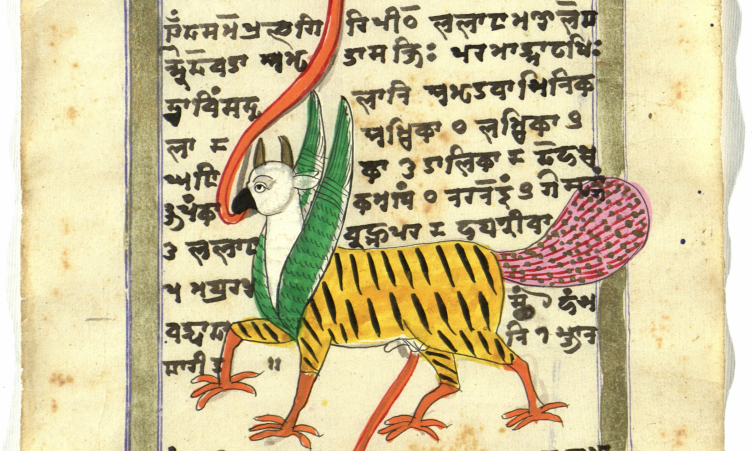
\includegraphics[width=1\textwidth]{pics/Wolpertinger.png}
\caption[The \textit{dehasvarūpa} of \textit{ajapāgāyatrī}]{The \textit{dehasvarūpa} of \textit{ajapāgāyatrī}. The image, reminiscent of a hippogriff, is part of an illustrated Sanskrit manuscript written in the Śāradā script. Preserved as a single large scroll under Acc. No. 1334 at the Oriental Institute in Srinagar (Kashmir), it is entitled \textit{Nāḍīcakra}. The manuscript contains a depiction of the yogic body’s \textit{cakra}s and \textit{nāḍī}s. The text surrounding the figure closely corresponds to the additional material found in manuscript \getsiglum{U2} of the \textit{Tattvayogabindu}. The manuscript reads (diplomatic transcription): \textit{oṃ daśame pūrṇagiripīṭhe lalāṭamaṇḍale candro devatā amṛtāśaktiḥ paramātmā ṛṣiḥ dvāviṃśaddalāni amṛtavāsinikalā 4: ambikā 1 lambikā 2 gha(ṃ)ṭkā 3 tālikā 4 dehasvarūpaṃ kākamukhaṃ 1 naranetraṃ 2 gośṛṅgaṃ 3 lalāṭabrahmapara 4 hayagrīvā 5 mayūramuśchaṃ 6 haṃsacārītani 7 sthāna.}}
	\phantomsection\label{fig_wolpertinger}
      \end{figure}

      \clearpage

  \begin{figure}[ht]
	\centering
  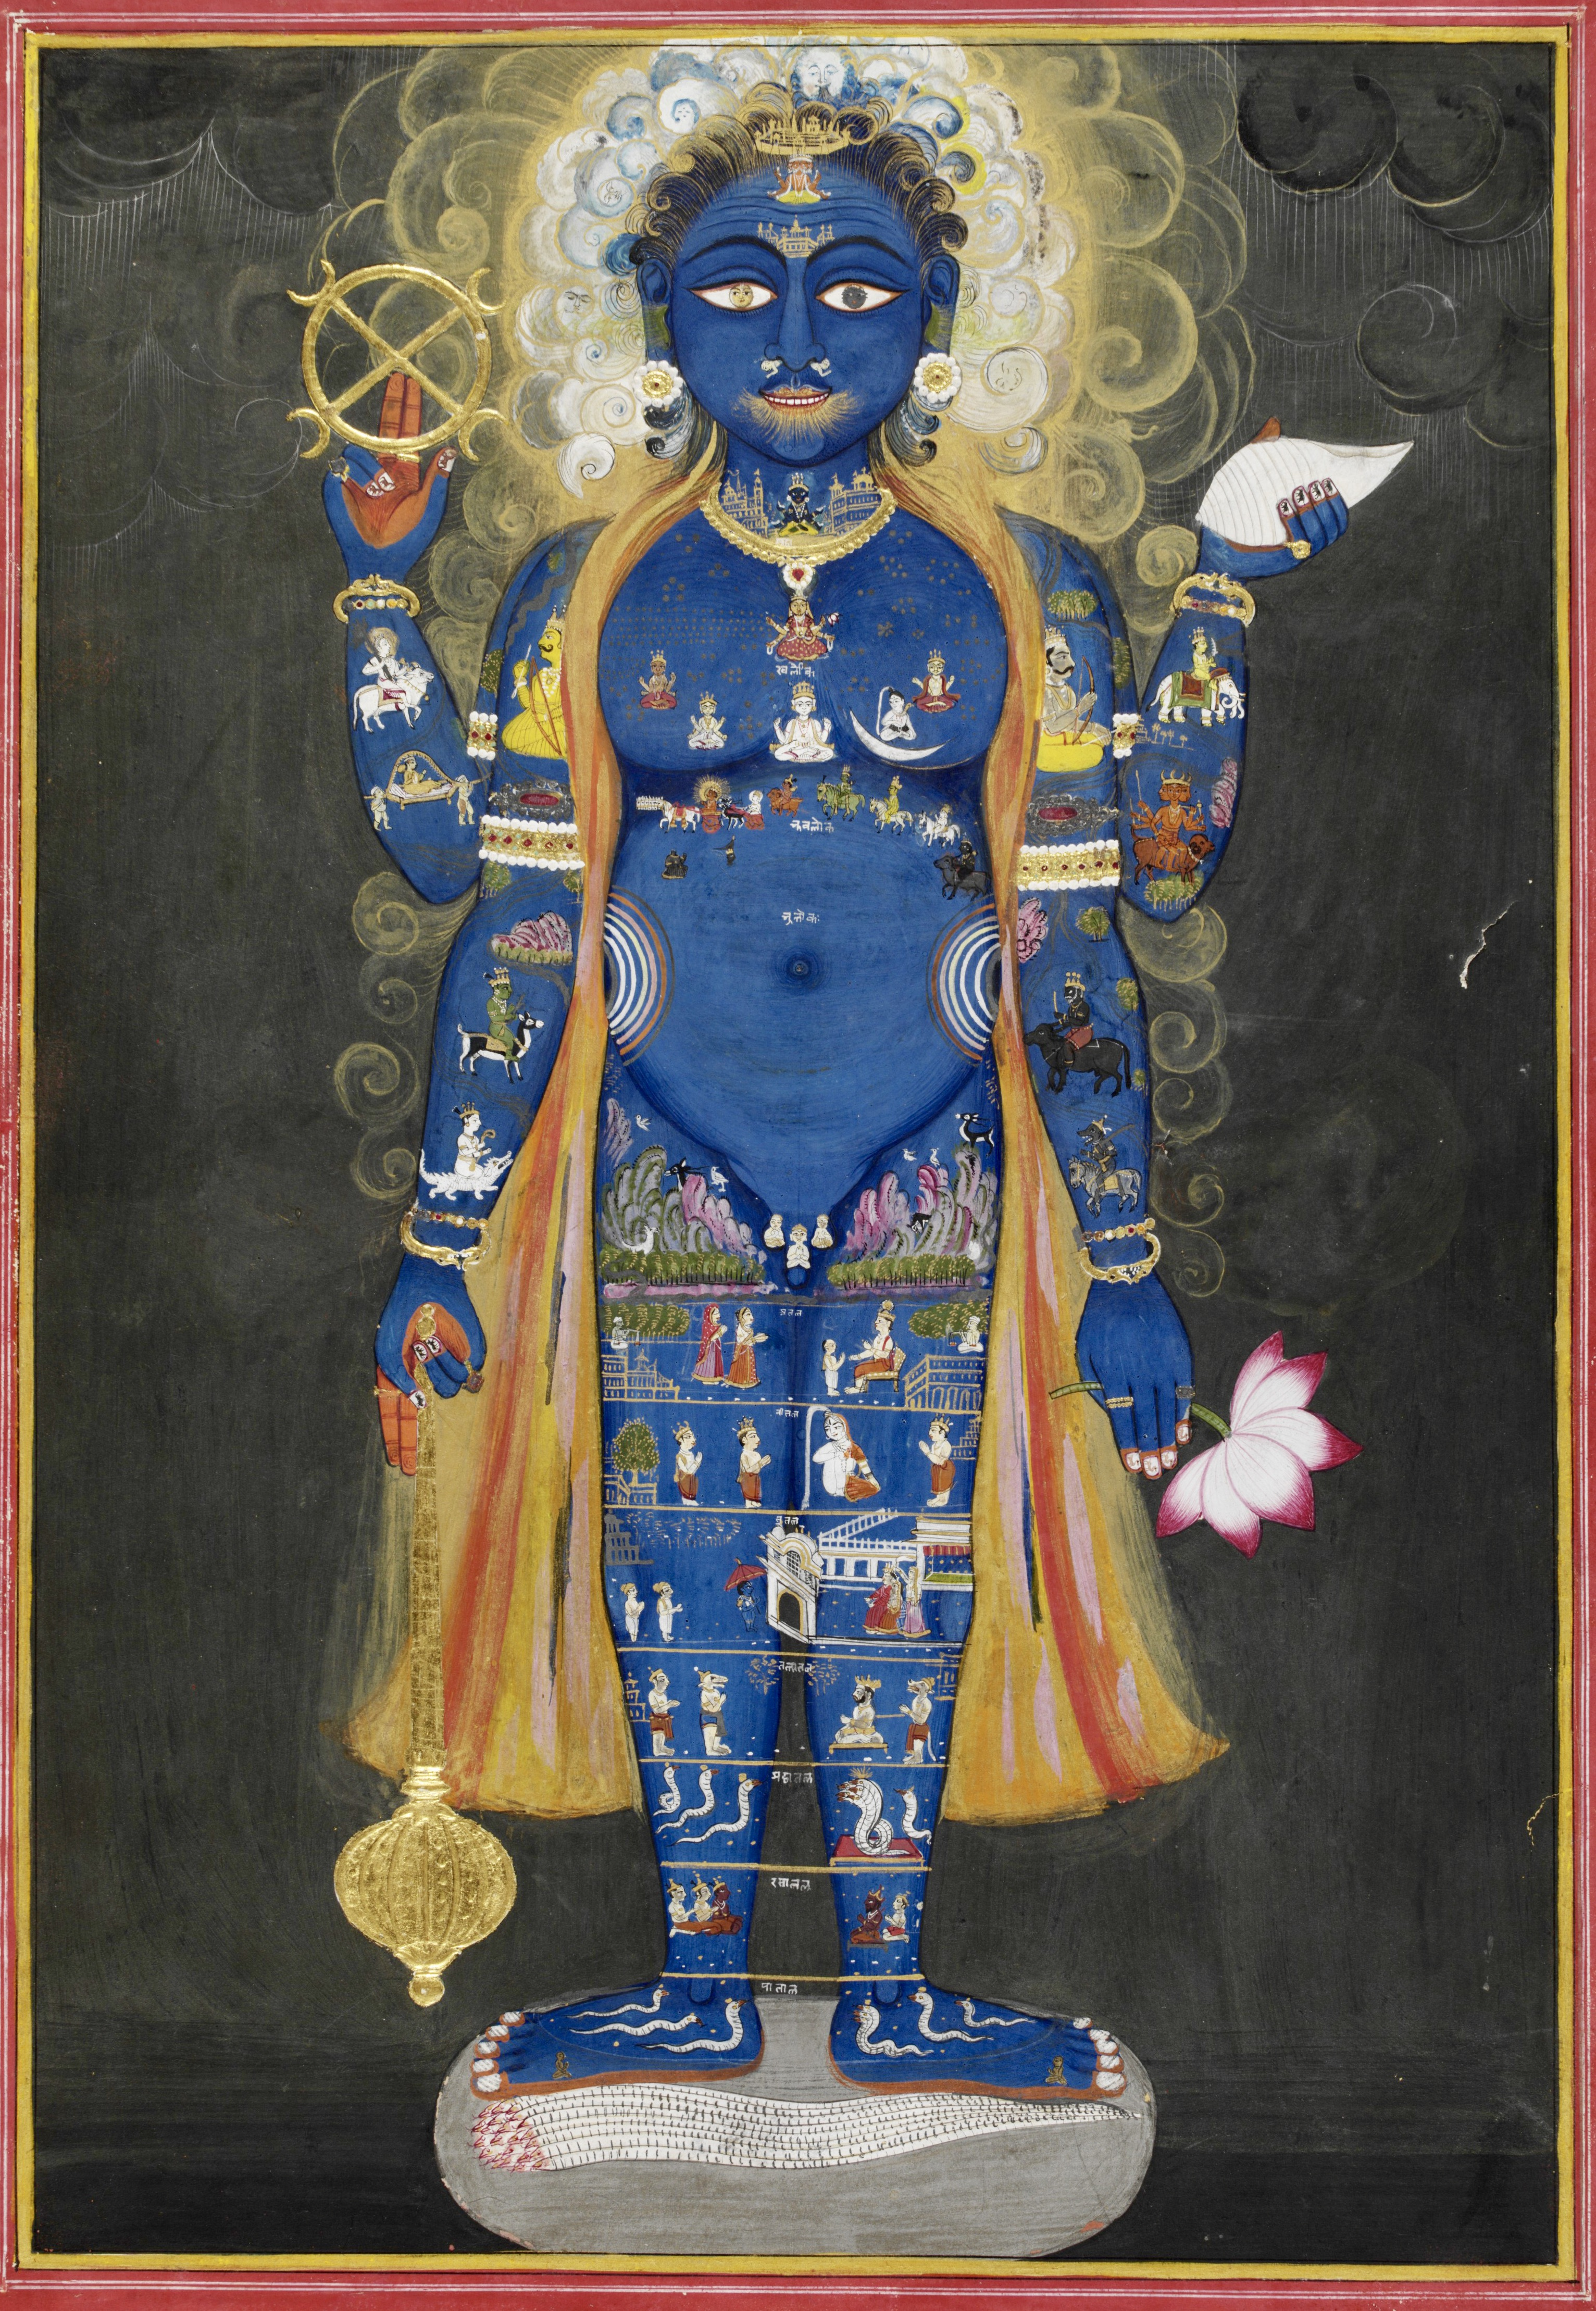
\includegraphics[width=1\textwidth]{pics/Vishnu_Vishvarupa_cropped.jpg}
	\caption{Viṣṇu Viśvarūpa, India, Rajasthan, Jaipur, ca. 1800–1820, Opaque watercolor and gold on paper, 38.5 × 28 cm, Victoria and Albert Museum, London, Given by Mrs. Gerald Clark.}
	\label{fig1}
      \end{figure}
\clearpage
  \begin{figure}[ht]
	\centering
  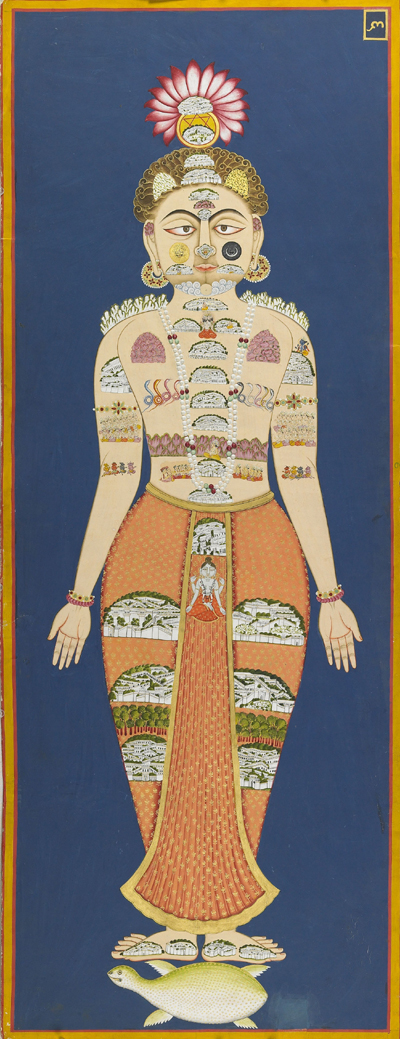
\includegraphics[width=0.5\textwidth]{pics/The_Equivalence_of_Self_and_Universe_(detail),_folio_6_from_the_Siddha_Siddhanta_Paddhati,_(Bulaki),_1824_(Samvat_1881);_122_x_46_cm._Mehrangarh_Museum_Trust..jpg}
	\caption{The Equivalence of Self and Universe (detail), folio 6 from the \textit{Siddhasiddhāntapaddhati} (Bulaki), India, Rajasthan, Jodhpur, 1824 (Samvat 1881), 122 x 46 cm, RJS 2378, Mehragarh Museum Trust.}
	\label{fig2}
      \end{figure}
      % \end{landscape}

      \newpage
      \cleardoublepage
\chapter{Bibliography}
 \label{sec:bibli}
\clearpage
\newpage 
\thispagestyle{empty}
\quad  \addtocounter{page}{-1}

\newrefcontext[sorting=tixel]
\printbibliography[heading=subbibintoc, title=Primary Sources, keyword=primary]

\newrefcontext[sorting=nyt]
\printbibliography[heading=subbibintoc, title=Secondary Literature, keyword=seclit]

\printbibliography[heading=subbibintoc, title=Catalogues, keyword=catalogues]

\printbibliography[heading=subbibintoc, title=Online Sources, keyword=onlinesource]

\end{document}
